% Source: TeX Live 2025, doc/generic/pgf/pgfmanual-en-tikz-plots.tex:723-731
% (xbar). Blue retains the four category positions and the manual's bar
% magnitudes, with two signs reversed. Teal is an added comparison series.
% Widths and grouping follow pgfmanual-en-library-plot-handlers.tex:379-393:
% both bands are 5pt thick; their centers are 4pt below/above each category.
\documentclass[border=2pt]{standalone}
\usepackage{tikz}
\begin{document}
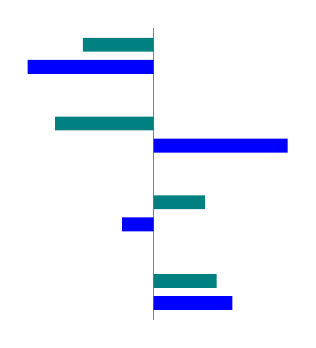
\begin{tikzpicture}
  \draw[gray] (0,-0.35) -- (0,3.35);
  \fill[blue,bar width=5pt,bar shift=-4pt] plot[xbar]
    coordinates {(1,0) (-0.4,1) (1.7,2) (-1.6,3)};
  \fill[teal,bar width=5pt,bar shift=4pt] plot[xbar]
    coordinates {(0.8,0) (0.65,1) (-1.25,2) (-0.9,3)};
\end{tikzpicture}
\end{document}
